\documentclass[prd,twocolumn,nofootinbib,superscriptaddress,amsmath,amssymb]{revtex4-1}
\usepackage{mathtools}
\usepackage{graphics}
\usepackage{graphicx}
\graphicspath{{./images/}}
\usepackage{dcolumn}
\usepackage{bm}
\usepackage{dsfont} 
\usepackage{amsmath,amssymb}
\usepackage{hyperref}
\usepackage{tabularx}
%\usepackage{epstopdf}
\usepackage{epsf,epsfig}
\usepackage[normalem]{ulem}
\usepackage[usenames]{color}
\usepackage{multirow}
\usepackage{makecell}
\usepackage{diagbox}
\usepackage[abs]{overpic}
%\epstopdfsetup{outdir=./images/}
\allowdisplaybreaks
\hypersetup{
    colorlinks=true,
    linkcolor=blue,
    filecolor=magenta,      
    urlcolor=blue,
    citecolor=blue
}
\urlstyle{same}


\newcommand{\red}[1]{\protect\color{red} #1 \protect\color{black}}
\newcommand{\green}[1]{\protect\color{green} #1 \protect\color{black}}
\newcommand{\blue}[1]{\protect\color{blue} #1 \protect\color{black}}
\newcommand{\black}[1]{\protect\color{black} #1 \protect\color{black}}
\newcommand{\yellow}[1]{\protect\color{yellow} #1 \protect\color{black}}
\newcommand{\bra}[1]{\protect\langle #1 |}
\newcommand{\ket}[1]{| #1 \protect\rangle}
\newcommand{\braket}[2]{\protect\langle #1 | #2 \protect\rangle}
\newcommand{\expected}[1]{\protect\langle #1 \protect\rangle}
\newcommand{\R}{{\mbox{\tiny R}}}
\newcommand{\ky}[1]{\textcolor{blue}{\it{\textbf{ky: #1}}} }
\newcommand{\kent}[1]{\textcolor{magenta}{\textbf{ #1}} }
\newcommand{\zack}[1]{\textcolor{magenta}{\textbf{ #1}} }
\newcommand{\zc}[1]{\textcolor{red}{\it{\textbf{zc: #1}}} }
\definecolor{red(ncs)}{rgb}{0.77, 0.01, 0.2}
\newcommand{\ny}[1]{\textcolor{blue}{NY: #1} }
\newcommand{\kc}[1]{\textcolor{green}{KC: #1} }
\newcommand{\NS}{{\mbox{\tiny NS}}}
\newcommand{\sci}[2]{#1 \times 10^{#2}}

\usepackage{array}
\newcolumntype{C}[1]{>{\centering\let\newline\\\arraybackslash\hspace{0pt}}m{#1}}


\newcolumntype{C}[1]{>{\centering\arraybackslash}m{#1}}

\def\eq#1{Eq.~(\ref{eq:#1})}
\def\Eq#1{Equation~(\ref{eq:#1})}
\def\eqs#1#2{Eqs.~(\ref{eq:#1}) \& (\ref{eq:#2})}
\def\eqlist#1#2{Eqs.~(\ref{eq:#1}-\ref{eq:#2})}
\def\Eqs#1#2{Equations~(\ref{eq:#1}) \& (\ref{eq:#2})}
\def\Eqlist#1#2{Equations~(\ref{eq:#1}-\ref{eq:#2})}
\def\fig#1{Fig.\ref{fig:#1}}
\def\figs#1#2{Figs.\ref{fig:#1} \& \ref{fig:#2}}
\def\Fig#1{Figure~\ref{fig:#1}}
\def\Figs#1#2{Figures~\ref{fig:#1} \& \ref{fig:#2}}
\def\tab#1{Table~\ref{tab:#1}}
\def\sec#1{Section~\ref{sec:#1}}



\definecolor{red(ncs)}{rgb}{0.77, 0.01, 0.2}
\newcommand{\ny}[1]{\textcolor{blue}{NY: #1} }
\newcommand{\kc}[1]{\textcolor{red}{KC: #1} }

\begin{document}

\title{Universal relations after GW170817}

\author{Frodo}
\affiliation{}

\author{Sam}
\affiliation{}

\author{Pippin}
\affiliation{}

\author{Merry}
\affiliation{}

\author{Gandalf}
\affiliation{}


\date{\today}

%%%%%%%%%%%%%%%%%%%%%%%%%%%%%%%% Begin Abstract %%%%%%%%%%%%%%%%%%%%%%%%%%%%%%%%%%%%%%%%%%%%%%%%%%%%%%%%%%%%%%%%%%%%%%%%%%%%%%%%%%%%%%%%%%%%%%%%%%%%%%%%%%%%%%%%%%%%%%%%%%%%%%%%%%%%%%%%%%%%%%%%%%%%%%%%%%%%%
\begin{abstract}
% Intro
The thermodynamic relationship between pressure and density (the equation of state) of supranuclear matter, accessible primarily in neutron stars, is critical to the study of such stars, and is one of the largest uncertainties in nuclear physics to date. 
% How to probe
The extraction of tidal deformabilities from the gravitational waveforms of binary neutron star merger events, such as GW170817, is a promising method of probing the nuclear structure.
% What was done before - Binary Love
Previous studies have shown that approximately equation of state insensitive ``binary Love universal relations" exist between symmetric and antisymmetric combinations of individual tidal deformabilities, which are difficult to be independently measured with second-generation gravitational wave interferometers.
% What was done before - I-Love-Q
Similarly, another set of equation of state independent relations exist between individual neutron star parameters: moment of inertia (I), tidal deformability (Love number), and quadrupole moment (Q) - known as the ``I-Love-Q universal relations."
% What universal relations do
Such universal relations allow the elimination of some tidal parameters from the list of model parameters, thus breaking degeneracies and ultimately reducing the uncertainty of the dominant tidal effect in parameter estimation.
% What we will do
In this document, we explain how one can reduce equation of state variation for both binary Love and I-Love-Q universal relations, which helps to reduce systematic errors on the tidal measurement of binary neutron star mergers. 
We achieve this  by restricting to only equations of state drawn within the 90\% posterior constraint on pressure as a function of density, as derived by the LIGO Collaboration.
% What we found
We find an improvement in binary Love universality by a factor of 25\% for stars with mass below 1.7 solar masses, and in I-Love-Q universality by a factor of 22\%\zc{check these numbers}.
% Conclude
We end by comparing systematic errors on tidal measurement due to the equation of state variation with statistical errors and comment on whether one can safely use these universal relations with future gravitational wave observations.
\end{abstract}

\maketitle

%%%%%%%%%%%%%%%%%%%%%%%%%%%%%%% Begin Introduction %%%%%%%%%%%%%%%%%%%%%%%%%%%%%%%%%%%%%%%%%%%%%%%%%%%%%%%%%%%%%%%%%%%%%%%%%%%%%%%%%%%%%%%%%%%%%%%%%%%%%%%%%%%%%%%%%%%%%%%%%%%%%%%%%%%%%%%%%%%%%%%%%%%%%%%%%%%%%%

\section{Introduction}\label{sec:intro}
%Intro
The dependance of pressure on density for supranuclear matter found primarily inside neutron stars (NSs) remains to be one of the largest mysteries in both nuclear physics and astrophysics.
This internal structure of such stars, known as the equation of state (EoS), is exceedingly important, as it is the determining factor for many NS observables - such as the mass, the radius, and many more.
Unfortunately, terrestrial experiments can only study the EoS up to the nuclear saturation density ($\rho_{\text{sat}} \approx 2.5 \times 10^{14} \text{ g/cm}^3$)~\cite{Li:HeavyIon,Tsang:SymmetryEnergy,Centelles:NeutronSkin,Li:CrossSections,Chen:SymEnergy}, making NSs ideal laboratories for constraining ultra dense nuclear matter.

%Constraining the EoS
Independent measurements of NS observables can be used to constrain the nuclear EoS.
For example, electromagnetic observations of the mass-radius relationship of NSs have been used to place limits on NSs~\cite{guver,ozel-baym-guver,steiner-lattimer-brown,Lattimer2014,Ozel:2016oaf}.
However, these implications suffer from large systematic errors due to astrophysical mismodeling.
Alternatively, the emission of gravtiational waves (GWs) from binary NS merger events have proven to be a unique method of probing nuclear physics.
During the early inspiral portion of the merger, the orbital separation is large enough that the effect of companion tidal fields is negligable. 
As the separation decreases through GW emission, tidal forces are magnified and the NSs deform from sphericity, altering the orbital trajectories; a relic which is directly imprinted on the GW signal.
This deformation is characterized by the \textit{tidal deformability} $\Lambda$ as the linear response of the NSs quadrupole moment $Q_{ij}$ to the neighboring tidal field $\varepsilon_{ij}$.

%reparameterization of the template
In the case of binary NSs, each star becomes deformed via the process highlighted above, resulting in two highly correlated tidal parameters $\Lambda_1$ and $\Lambda_2$ entering in the gravitational waveform.
Due to high correlations between between the two paramters, independant extraction becomes very difficult at current interferometer sensitivities.\zc{cite?}
Typically, these high correlations can be reduced by strategically reparameterizing the waveform template with new tidal parameters constructed from linear combinations of $\Lambda_1$ and $\Lambda_2$.
For example, utilizing the parameters $\tilde{\Lambda}$ and $\delta \tilde{\Lambda}$~\cite{hinderer-love,Flanagan2008} which enter the GW waveform at different post-Newtonian (PN) orders (powers of the ratio between the orbital speed and the speed of light $v/c^{2n}$) partially mitigates these correlations.

%Universal relations
Unfortunately, current detectors are only sensitive enough to accurately measure the dominant tidal parameter, $\tilde{\Lambda}$, known as the chirp deformability.
Previous work by Yagi and Yunes~\cite{Yagi:binLove} resolved this issue by finding approximately EoS-insensitive ``binary Love universal relations" between symmetric and anti-symmetric combinations of tidal deformabilities $\frac{1}{2}(\Lambda_1 \pm \Lambda_2)$.
This allows one to further break degeneracies between tidal parameters, resulting in both (i) a decrease in uncertainty upon parameter extraction on the removal of one parameter from the model, and (ii) the ability to measure the secondary tidal parameter upon measurement of the first.  
This important work showed up to an order of magnitude improvement in parameter estimation through a simple Fisher analysis.
Similar ``I-Love-Q" universal relations~\cite{Yagi:ILQ} have been found between individual NS observables: quadrupole moment , moment of inertia, and tidal deformability; similarly allowing the removal of tidal parameters from the model list, and allowing an automatic determination of one observable through the measurement of another.

%How we improved this
In this analysis, we aim to improve this important work by imposing the restrictions found on the EoS~\cite{LIGO:posterior} derived from the recent binary NS merger observation, GW170817~\cite{TheLIGOScientific:2017qsa}.
By restricting to only EoSs which lie within the the 90\% credible region on pressure as a function of density found in~\cite{LIGO:posterior}, we repeat the analyses done in~\cite{Yagi:binLove,Yagi:ILQ} and show an increase in universality for both binary Love and I-Love-Q universal relations.
In addition, we consider hybrid star EoSs seen in~\cite{Paschalidis2018}, which experience strong first-order transitions from hadronic matter to quark matter.
These provide a departure from the nuclear matter relations considered here - providing valuable insight into them.
Further, we estimate the viability of using improved universal relations on future GW detections by performing simple Fisher analyses to approximate when the statistical errors from parameter extraction become comparable to the systematic errors due to EoS variation in universal relations.

\subsection{Executive Summary}
%What we did
In this paper we attempt to improve binary Love and I-Love-Q universal relations by imposing constraints on the EoS found by GW170817~\cite{LIGO:posterior,TheLIGOScientific:2017qsa}.
First, we generate two large samples of spectral EoSs~\cite{Lindblom:2018rfr}, where we (i) impose the restriction that they must lie within GW170817's 90\% credible region in pressure as a function of density, and (ii) don't impose any restrictions for comparison purposes.
Next, we follow the important works of~\cite{Yagi:binLove} and~\cite{Yagi:ILQ} to show how the ``constrained" set of EoSs show improved universality from both the previous works, and the ``unconstrained" sample.
In addition, we determine the degree to which hybrid star EoSs obey binary Love universal relations.
Lasty, through a simple Fisher analysis, we consider the value in improving universal relations by approximating when the statistical errors from parameter extraction become comparable to the systematic errors due to EoS variation in universal relations.

%Final Results
Upon use of the constrained set of EoSs, we find an improvement in binary Love universality by a factor of 25\% for stars with mass below 1.7 solar masses, and in I-Love-Q universality by a factor of 22\%.
We also find that binaries consisting of one massive hybrid star, and one small-mass hadronic star do not agree with derived binary Love relations, due to the large separation in $\tilde{\Lambda}$ between the constituent stars.
Unfortunately, due to the current limitations in detector sensitivity, the systematic errors arising from EoS variation in the universal relations are far outweighed by the statistical errors accrued by extraction of high-order PN tidal parameters from GW waveforms.
Fig.~\ref{fig:stackedFisher} compiles the results from Fisher analyses approximating the uncertainties accrued from parameter extraction for GW170817 as if it had been observed by future detectors $A \equiv ($ O2, aLIGO, a\texttt{++}, Voyager, ET, CE$)$\zc{cite these individually}.
Here, $\sigma^A_{\text{GW170817}}$ and $\rho^A_{\text{GW170817}}$ correspond to the statistical error and signal-to-noise-ratio found from observing GW170817 on detector $A$, and $\sigma^A_N$ represents the combined uncertainty after the detection of $N_A$ events (corresponding to the binary NS merger rate associated interferometer $A$).
These values are further tabulated in Table~\ref{tab:variances}.
It can be seen from this figure that the statistical errors from parameter extraction become comparable the universal relation systematics (indicated by the magenta horizontal line) for the Voyager telescope - indicating when improved binary Love universal relations will become viable.
\begin{figure}
\begin{center} 
\includegraphics[width=\columnwidth]{stackedFisher.eps}
\end{center}
\caption{
Estimated statistical uncertainties $\sigma^A_{\text{GW170817}}$ (blue) in the extraction of $\tilde{\Lambda}$ from GW170817 (O2) as if observed with future interferometers aLIGO, a++, Voyager, CE, and ET-D as a function of the signal-to-noise-ratio $\rho^A_{\text{GW170817}}$.
This is compared to the combined uncertainty $\sigma^A_N$ (red) from the observation of multiple events from a simulated population of size $N_A$ corresponding to the upper (teal), central (orange), and lower (magenta) limits of expected binary NS merger detection rates for O2, aLIGO, a\texttt{++}, Voyager, CE, and ET-D over 1 observation year.
It can be seen that the statistical errors in parameter extraction become comparable to the systematics from EoS variation in binary Love relations (purple) for Voyager and on.
Note the approximation for $\sigma^A_N$ under the O2 detector sensitivity is a poor estimate due to the small number of stacked events, $N_{\text{O2}}=1$, resulting in a high degree of randomness in population generation.
These results are further tabulated in Table~\ref{tab:variances}.
}
\label{fig:stackedFisher}
\end{figure} 

%outline
The organization of this paper is outlined below.
We begin with a complementary background and theory material in Sec.~\ref{sec:theory}.
We continue in Sec.~\ref{sec:universal} by finding new and improved binary Love and I-Love-Q universal relations, and considering how well hybrid star EoSs agree with the binary Love relations.
We next examine these improved universal relations and question whether or not they are useful for future interferometers in Sec.~\ref{sec:observations}.
We conclude in Sec.~\ref{sec:conclusion} by discussing our results and mentioning avenues of future work.
Throughout this paper, we have adopted geometric units of $G=c=1$, unless otherwise stated.

%%%%%%%%%%%%%%%%%%%%%%%%%%%%%%%%% Begin theory %%%%%%%%%%%%%%%%%%%%%%%%%%%%%%%%%%%%%%%%%%%%%%%%%%%%%%%%%%%%%%%%%%%%%%%%%%%%%%%%%%%%%%%%%%%%%%%%%%%%%%%%%%%%%%%%%%%%%%%%%%%%%%%%%%%%%%%%%%%%%%%%%%%%%%%%%%%%
\section{Background and theory}\label{sec:theory}

\subsection{Spectral representations of neutron star equations of state}\label{sec:eos}
The structure of a NS and its tidal interactions in a binary system rely heavily on the underlying state function describing the relationship between pressure ($p$) and energy density ($\epsilon$), or equation of state, of nuclear matter.
Given that all currently proposed EoSs utilize certain approximations, one method to study a wide range of physically realizeable EoSs is to parameterize them in a model-independent way.
Spectral representations~\cite{Lindblom:2010bb,Lindblom:2012zi,Lindblom:2013kra,Lindblom:2018rfr,Abbott:2018exr} parameterize EoSs by performing spectral expansions on the adiabatic index $\Gamma(p)$\footnote{Another way of parameterizing EoSs is the piecewise polytropic formulation~\cite{Read2009,Lackey:2014fwa,Carney:2018sdv}.}:
\begin{equation}
\Gamma(x) = \exp{\sum_k\gamma_k x^k},
\end{equation}
where $x \equiv \log{p/p_0}$ for minimum pressure $p_0$.
The equation of state is then determined by an integration of the differential equation:
\begin{equation}
\frac{d \epsilon(p)}{dp}=\frac{\epsilon(p)+p}{p \Gamma(p)}.
\end{equation}
Using this formalism, any valid EoS can be approximated through choice of 4 or more spectral coefficients $\gamma_k$, tabulated for several common EoSs in Table 1 of~\cite{Lindblom:2018rfr}.

In the current analysis, we consider only EoSs which have been constrained by the recent binary neutron star merger event, GW170817.
Important recent work~\cite{LIGO:posterior} uniformly sampled EoS parameters in order to derive a marginalized posterior on the pressure as a function of mass density, as seen in Fig. 2 of~\cite{LIGO:posterior}.
In our work, we similarly sample spectral coefficients within the ranges: $\gamma_0 \in \lbrack 0.2,2 \rbrack$, $\gamma_1 \in \lbrack -1.6,1.7 \rbrack$, $\gamma_2 \in \lbrack -0.6,0.6 \rbrack$, $\gamma_0 \in \lbrack -0.02,0.02 \rbrack$, and further restricting the adiabatic index to be $\Gamma \in \lbrack 0.6,4.5 \rbrack$, ensuring our parameterization exposes a wide range of viable EoSs~\cite{Lindblom:parameters}.
In addition, we impose similar constraints as was done in~\cite{LIGO:posterior}: (i) causality within 10\%, and (ii) EoS priors must support NS masses up to $1.97 \text{ M}_{\odot}$, consistent with astrophysical observations.
We then utilize the posterior defined by GW170817 by rejecting any EoS sample which does not lie within the 90\% credible posterior region, resulting in a sample of 35 EoSs shown in Fig.~\ref{fig:eos}.
\kc{Why aren't we directly using the gamma's that Carl provided?}
Following~\cite{Read2009}, the parameterized high-density core EoSs generated above are matched to the low-density crust EoS Sly~\cite{Douchin:2001sv} at about half of the nuclear saturation density, $\rho_{\text{stitch}}=1.3 \times 10^{14} \text{ g/cm}^3$.
For comparison, we also include a second sample of randomly generated EoSs, without restricting to GW170817s posterior. {\ny{It would be good to make this figure a double pane one, so that you can show the constrained set and the unconstrained set side-by-side.}}
\begin{figure}
\begin{center} 
\includegraphics[width=\columnwidth]{EoSs.eps}
\end{center}
\caption{
Representative set of EoSs used in our analysis. 
These were populated by uniformly sampling the spectral coefficient parameter space, then restricting to the 90\% credible level shown in cyan~\cite{LIGO:posterior}.
In addition, the following constraints were also applied: (i) the EoS must have a causal structure within 10\%, and (ii) the EoS must support maximum NS mass of at least $1.97 \text{ M}_{\odot}$, consistent with astrophysical observations.
Finally, the high density core EoSs generated above were stitched to the low-density crust EoS of SLy~\cite{Douchin:2001sv} at $\rho_{\text{stitch}}=1.3 \times 10^{14} \text{ g/cm}^3$.
}
\label{fig:eos}
\end{figure} 

\subsection{Neutron Star Tidal deformability}\label{tidal}
Binary neutron star mergers, such as GW170817, provide valuable insight into the internal structure of such stars. 
Namely, tidal effects which enter the gravitational waveform depend strongly on the EoS defining the NSs structure. 
The ($l=2$ electric type) \emph{tidal deformability}, denoted as $\lambda$, has the largest impact on the waveform phase. 
Consider a NS of mass $M$ in the presence of the tidal field $\varepsilon_{ij}$ of a companion star.
In response, the NS will deform away from sphericity under the aquisition of quadrupole moment $Q_{ij}$, characterized by $\lambda$ as the linear response to $\varepsilon_{ij}$~\cite{Flanagan2008,hinderer-love,Yagi2013}:
\begin{equation}
Q_{ij}=-\lambda \varepsilon_{ij}.
\end{equation}
One can extract $Q_{ij}$ and $\varepsilon_{ij}$ -- and thus $\lambda$, or its dimensionless form $\Lambda \equiv \lambda/M^5$ -- via diffent asymptotic limits of the gravitational potential:
\begin{align}
\begin{split}
\Phi=\frac{1+g_{tt}}{2}&=-\frac{M}{r} - \frac{3}{2}\frac{Q_{ij}}{r^3} \Bigg(\frac{x^i}{r} \frac{x^j}{r}-\frac{1}{3}\delta_{ij} \Bigg) + \mathcal{O} \Bigg( \frac{M^4}{r^4} \Bigg)\\
&+ \frac{1}{2} \varepsilon_{ij} x^i x^j + \mathcal{O} \Bigg( \frac{r^3}{M^3} \Bigg).
\end{split}
\end{align}
The metric component $g_{tt}$ is determined by first constructing a spherically symmetric, non-spinning background solution, followed by the introduction of a perturbative tidal deformation.
Next, the perturbed Einstein equations must be solved in the NSs interior given an EoS, then matched to the exterior Schwarzschild solution at the surface, modulo a constant.
This process is described in more detail in Ref.~\cite{hinderer-love}.
Further, the stellar mass and radius are determined from $p(R)=0$, and the above mentioned constant.
Similarly, the moment of inertia is obtained from the asymptotic behavior of the $g_{t \phi}$ metric component.

Next, we consider the case of two NSs in a binary, such as the system found in GW170817, where each star 
individually experiences a neighboring tidal field.
Thus each star possesses tidal deformabilities $\Lambda_1$ and $\Lambda_2$ entering the gravitational waveform.
Due to strong correlations between these parameters, individual extraction is very difficult with current interferometer sensitivity limitations.
However, the waveform templates can be strategically reparameterized to instead include independant linear combinations of $\Lambda_1$ and $\Lambda_2$ to mitigate correlations between them. 
Any set of two independent functions may be used, for example: tidal parameters $\tilde{\Lambda}=\tilde{\Lambda}(\Lambda_1,\Lambda_2)$ and $\delta \tilde{\Lambda}=\delta \tilde{\Lambda}(\Lambda_1,\Lambda_2)$~\cite{Wade:tidalCorrections} first enter the gravitational waveform at 5PN and 6PN orders respectively, thus partially breaking degeneracies.
Here, $\tilde{\Lambda}$ is known as the mass weighted tidal deformability, or \emph{chirp deformability} due to its status as the dominant tidal parameter in the waveform. 

\subsection{EoS insensitive relations}\label{sec:eosInsensitive}
Current gravitational wave interferometry is not yet sensitive enough to accurately extract both tidal parameters $\tilde{\Lambda}$ and $\delta\tilde{\Lambda}$.
In a search to remedy this, important previous work by Yagi and Yunes~\cite{Yagi:binLove} found that symmetric and antisymmetric combinations of tidal deformabilities:
\begin{equation}
\Lambda_s \equiv \frac{\Lambda_1 + \Lambda_2}{2}, \hspace{6mm} \Lambda_a \equiv \frac{\Lambda_1 - \Lambda_2}{2},
\end{equation}
display EoS-insensitive properties to a high degree, showing EoS variations up to 20\% for binaries with masses less than $1.7 \text{ M}_{\odot}$, for a representative set of 11 EoSs. 
These relations, known as ``binary Love universal relations" allows one to break degeneracies between coupled tidal parameters.
This is important for two reasons: (i) allows us to algebraically eliminate tidal parameters from the template parameter list, improving parameter estimation, and (ii) automatic measurement of second tidal parameter given observation of the first.
It was shown through a simple Fisher analysis that the use of binary Love universal relations improved parameter extraction on $\tilde{\Lambda}$ by an order of magnitude.

Similal universal relations have been found to exist between individual NS observables: moment of inertia (I), tidal deformability (Love), and quadrupole moment (Q), known as the ``I-Love-Q" universal relations~\cite{Yagi:ILQ}.
These have been found to be EoS insensitive by up to 1\% for each of pair of observables.
In this paper, we show improvement in both of these universal relations by restricting to EoSs drawn within GW170817s posterior on pressure as a function of density.
%%%%%%%%%%%%%%%%%%%%%%%%% Begin universal relations %%%%%%%%%%%%%%%%%%%%%%%%%%%%%%%%%%%%%%%%%%%%%%%%%%%%%%%%%%%%%%%%%%%%%%%%%%%%%%%%%%%%%%%%%%%%%%%%%%%%%%%%%%%%%%%%%%%%%%%%%%%%%%%%%%%%%%%%%%%%%%%%%%%%%
\section{Universal relations}\label{sec:universal}
In this section, we follow the analyses performed in~\cite{Yagi:binLove,Yagi:ILQ} with two new sets of 35 spectrally generated EoS: (i) those constrained by GW170817s 90\% credible region on pressure as a function of density as shown in Fig.~\ref{fig:eos}, and (ii) those unconstrained by any prior information.
For the remainder of the paper, we refer to these distinct samples as ``constrained" and ``unconstrained." 

\subsection{I-Love-Q relations}\label{sec:ilq}
Here we present our results on I-Love-Q universality as compared to Fig. 1 of Yagi and Yunes~\cite{Yagi:ILQ}.
Following this work, the data for each universal relation is fit to the following curve:
\begin{equation}\label{eq:ILQfit}
\ln{y_i}=a_i+b_i \ln{x_i} + c_i (\ln{x_i})^2 + d_i (\ln{x_i})^3 + e_i (\ln{x_i})^4,
\end{equation}
where the updated coefficients are given in Table~\ref{tab:ILQfit}.
In particular, we focus only on the I-Love universal relation for brevity, noting that the remaining relations Q-Love and I-Q show similar results.

\begin{table}[ht!]
\centering
\caption{
Updated fit parameters for I-Love-Q universal relations, as given by the curve found in Eq.~\ref{eq:ILQfit}.
}\label{tab:ILQfit}
\begin{tabular}{ c  c | c c c c c } 
 \hline
 \hline
 $y_i$ & $x_i$ & $a_i$ & $b_i$ & $c_i$ & $d_i$ & $e_i$ \\
 \hline
 $\bar{I}$ & $\Lambda$ & $1.49$ & $0.0632$ & $0.0212$ & $-5.47 \times 10^{-4}$ & $2.18 \times 10^{-6}$ \\
 $\bar{I}$ & $\bar{Q}$ & $0.212$ & $0.0726$ & $0.0542$ & $-5.07 \times 10^{-3}$ & $1.60 \times 10^{-4}$ \\
 $\bar{Q}$ & $\Lambda$ & $1.38$ & $0.590$ & $-0.0183$ & $0.0405$ & $-2.77 \times 10^{-3}$ \\ 
 \hline
 \hline
\end{tabular}
\end{table}

{\ny{Let me play devil's advocate and explain things I could potentially be worried about.
\begin{itemize}
\item The constrained and the unconstrained data set of I-Love that you are fitting, do they have the same number of data points? If not, how do you know your fits and the comparisons are reliable to variation on the data set? You can study this by re-doing this analysis with the same amount of data in both sets of EoSs and then repeating the analysis with twice the amount of data to see how the results change.  
\item  The unconstrained set does not contain the same EoSs as the constrained set plus additional ones that are ruled out. This makes comparison of the sets a bit more difficult, because they are randomly sampled. How do you know your comparisons are robust to the number of EoSs you have randomly chosen without your probability distribution? You can study this by re-doing this analysis with twice the number of drawn EoSs to see how the results change. 
\item In the constrained set, there seems to be 3 EoSs that have the ``largest'' difference. What makes these EoSs special? Do they have anything in common?  Same question for the unconstrained data set, but there are 2 special ones this time. 
\end{itemize}
}}
Fig.~\ref{fig:ILQ} shows the improved I-Love universal relation between dimensionless moment of inertia $\bar{I} \equiv I/M^3$ and dimensionless tidal deformability $\Lambda$ for both constrained and unconstrained sets of EoSs.
We observe that the maximum recorded EoS variation under the constrained set of EoSs is $0.43\%$, showing considerable improvement from the $0.88\%$ found in the case of unconstrained EoSs.
Further, both EoS samples show improvement from the original result of $\approx 1\%$ displayed in~\cite{Yagi:ILQ}.

{\ny{This comment is related to the list above, but I'm worried about how robust these numbers quoted above to *2* sig figs are...}}

\begin{figure*}
\begin{center} 
\includegraphics[width=\textwidth]{ILQ.eps}
\end{center}
\caption{
I-Love universal relations shown for the constrained EoSs (left) and unconstrained EoSs (right).
In these figures, the black dashed lines corresponds to the fit given by Eq.~\ref{eq:ILQfit}, while all other colors correspond to the 35 EoSs used in each case.
The maximal EoS variation from the fit for unconstrained EoSs is $0.88\%$, which is comparable to the $1\%$ found in~\cite{Yagi:ILQ}.
The constrained EoSs on the other hand, are universal to $0.43\%$, showing considerable improvement upon previous analyses.
}
\label{fig:ILQ}
\end{figure*} 

These results indicate that universal relations can indeed be improved upon by constraining to only EoSs that agree with physical observations.
Although the unconstrained EoSs show slightly smaller EoS variation than found in previous works, they are comparable in the sense that a wide range of EoSs were strategically picked in~\cite{Yagi:ILQ}, while the unconstrained set consists of a random sample which may or may not encompass everything considered previously.
On the other hand, the constrained set of EoSs show significant improvement from that found in previous 
works.

{\ny{I think it would be worth studying whether there is a better fitting function that one can use for the constrained set. The functional form in Eq. (6) does not limit properly to the Newtonian result or to the relativistic result. But we do know how I-Love for example scales in the Newtonian limit, so could we e.g. peel off the asymptotic behavior analytically, and then correct this with a fitting function? This is similar to what Kent and I did in the past in a paper (in the binary love actually) and also similar to the way EoB works.}}

\kc{why not study the I-Q relation too?}
\subsection{Binary love relations}\label{sec:binary}
Next we consider improvements to the binary Love universal relations.
In particular, we consider two distinct classes of NSs: nuclear matter EoSs and hybrid quark-hadron star EoSs~\cite{Paschalidis2018,Alford:2017qgh,1971SvA....15..347S,Zdunik:2012dj,Alford:2013aca}.
In the latter, the low-density nucleonic crust region of the EoS experiences a first-order phase transition into a high density quark matter core at a given transition pressure $P_{\text{tr}}$.
In this document, we adopt the ACB models, in particular ACB5 as seen in Table II of Ref.~\cite{Paschalidis2018}.
We begin in Sec.~\ref{sec:nuclear} by fitting new binary Love relations for nucleonic matter as was done in~\cite{Yagi:binLove}.
This is followed in Sec.~\ref{sec:hybrid} by an analysis and discussion into how well hybrid stars agree with the improved binary Love relations

{\ny{Why do we consider hybrid stars only in this subsection? Why not also include these in the I-Love studies?}}

\subsubsection{Nuclear matter stars}\label{sec:nuclear}
Following Ref.~\cite{Yagi:binLove}, we fit the binary Love relations from the constrained EoSs to the two-dimensional curve:
\begin{equation}\label{eq:binLovefit}
\Lambda_a=F_n(q) \frac{a+ \sum_{i=1}^3 \sum_{j=1}^2 b_{ij}q^j x^{i/5}}{a+ \sum_{i=1}^3 \sum_{j=1}^2 c_{ij}q^j x^{i/5}} \Lambda_s^{\alpha},
\end{equation}
where q is the mass ratio $q \equiv m_1/m_2$ with $m_1 \leq m_2$, and $F_n(q)$ being the Newtonian limit given by:
\begin{equation}
F_n(q) \equiv \frac{1-q^{10/(3-n)}}{1+q^{10/(3-n)}}.
\end{equation}
The updated fit parameters can be found in Table~\ref{tab:binLovefit}.
Notice how, unlike the individual NS I-Love-Q universal relations, these relations also depend on the ratio of constituent masses in the binary system.
\begin{table*}[ht!]
\centering
\caption{
Updated fit parameters for the binary Love universal relations, as given by the curve found in Eq.~\ref{eq:binLovefit}.
}\label{tab:binLovefit}
\addtolength{\tabcolsep}{1pt} 
\begin{tabular}{ c  c  c  c  c  c  c  c  c  c  c  c  c  c  c} 
 \hline
 \hline
 $n$ & $\alpha$ & $a$ & $b_{11}$ & $b_{12}$ & $b_{21}$ & $b_{22}$ & $b_{31}$ & $b_{32}$ & $c_{11}$ & $c_{12}$ & $c_{21}$ & $c_{22}$ & $c_{31}$ & $c_{32}$\\
 \hline
 $0.743$ & $-1$ & $0.08684$ & $-2.594$ & $-0.6145$ & $9.659$ & $3.024$ & $-7.816$ & $17.5488$ & $-2.172$ & $-1.744$ & $3.609$ & $18.14$ & $11.45$ & $-29.90$\\
\hline
 \hline
\end{tabular}
\addtolength{\tabcolsep}{-1pt}
\end{table*}

Fig.~\ref{fig:binLove} shows the improved binary Love universal relation for 3 different mass ratios: $q=0.9$, $q=0.75$, and $q=0.5$ for both constrained and unconstrained sets of EoSs.
We observe that the maximum recorded EoS variation under the constrained set of EoSs is $23.65\%$, $9.76\%$, and $2.15\%$ for mass ratios of $q=0.9$, $q=0.75$, and $q=0.50$, respectively.
This shows considerable improvement from the universalities of $\sim 50\%$, $\sim 20\%$, and $\sim 3\%$ found in Ref.~\cite{Yagi:binLove}.
In addition, the unconstrained set of EoSs show similar universality to that recorded in Ref.~\cite{Yagi:binLove}.
\begin{figure*}
\begin{center} 
\includegraphics[width=\textwidth]{binLove.eps}
\end{center}
\caption{
Binary Love universal relations shown for the constrained EoSs (left) and unconstrained EoSs (right).
In this figure, the dashed black line corresponds to the fit given by Eq.~\ref{eq:binLovefit}, while the dotted blue, dashed magenta, and solid green lines represent the 35 EoSs for mass ratios of $q=0.9$, $q=0.75$, and $q=0.50$, respectively.
The maximal EoS variation for each value of $q$ is $23.65\%$, $9.76\%$, and $2.15\%$ respectively, compared to $\sim 50\%$, $\sim 20\%$, and $\sim 3\%$ found in Ref.~\cite{Yagi:binLove}.
These values are comparable to the maximal EoS variation for unconstrained EoSs as expected, found to be $41.66\%$, $12.64\%$, and $3.83\%$.
Additionally shown is the binary Love relations for hybrid stars (dash-dash-dotted curves) as discussed in Sec.~\label{sec:hybrid}.
Observe the large deviations from the fit as the mass ratio $q$ increases, returning near the fit before the transitional pressure at large values of $\Lambda_s$.
}
\label{fig:binLove}
\end{figure*} 

{\ny{I have very similar comments here to those I listed in the I-Love relation section.}}

\subsubsection{Hybrid quark-hadron stars}\label{sec:hybrid}
\begin{figure}
\begin{center} 
\includegraphics[width=\linewidth]{hybridML.eps}
\end{center}
\caption{
$M-\tilde{\Lambda}$ relations for the ACB5 model hybrid star. 
Note the strong phase transition into a quark-matter branch at $\sim 1.4 \text{ M}_{\odot}$.
As described in the text, HS/HS and NS/NS binaries have individual masses chosen such that both stars are contained within one branch -- resulting in high $q$ values.
Constrastingly, HS/NS binaries have individual masses chosen from each branch resulting in small $q-values$.
}
\label{fig:hybridML}
\end{figure} 
Transitional quark-hadron matter stars undergo first-order phase transitions at pressure $P_{\text{tr}}$, where the hadronic branch departs into a quark-matter branch at a given mass transition.
We focus on the ACB5 model shown in Fig.~\ref{fig:hybridML}, which observes a transition mass at $\sim 1.4 \text{ M}_{\odot}$~\cite{Paschalidis2018}.
This results in two distinct types of NSs, based on their observed mass: (i) massive ($M \geq 1.4 \text{ M}_{\odot}$) hybrid stars which have quark-matter cores and nuclear matter crusts (we denote this as ``HS"), and (ii) small-mass ($M \leq 1.4 \text{ M}_{\odot}$) hadronic stars with no internal transition to quark matter (we denote this as ``NS").
We consider 3 classes of binaries:
\begin{itemize}
\item HS/NS binary: consists of one massive hybrid star, and one small hadronic neutron star,
\item NS/NS binary: consists of two small-mass hadronic neutron stars,
\item HS/HS binary: consists of two massive hybrid stars.
\end{itemize}

{\ny{The comparison below is a bit misleading because all you have shown is that the fitting coefficients for the standard stars do not work when dealing with mixed stars. I think it would be interesting to see how the binary love relations look when you include hybrid systems (something like Fig. 5 but for QS/QS and for QS/HS). Also I think it would be interesting to either (i) redo the fits including the QS/QS and QS/HS data and or (ii) produce different fits for those families, and then you can compare either of these to a wide set of systems to determine the validity of the fit.}}

To determine how each of class of binary NSs obey our improved binary Love universal relations, we pick a representative set of 10 binary pairs from each class.
Binary Love values are then computed for each pair, then residuals from the binary Love curve found in Sec.~\ref{sec:nuclear} are determined and compared to that from the constrained set of EoSs.
The results are shown in Fig.~\ref{fig:hybrid}.
First, we observe that the NS/NS combination of stars gives consistent results to that found earlier -- as expected.
Next, we see that HS/HS combinations agree moderately with previous relations\footnote{Note that these EoSs do not fit within GW170817's 90\% posterior on EoS - so we excpect deviations consistent with the ``unconstrained" set of EoSs, rather than the ``constraind" set.}, while HS/NS combinations disagree significantly.
This can be explained by the large reduction in tidal deformability for hybrid stars, are shown in Fig. 2 of Ref.~\cite{Paschalidis2018}: when one star lies on the hadronic branch while the other is on the quark branch, they each see vast differences in $\tilde{\Lambda}$ - disrupting the binary Love relations as found for stars on the hadronic branch.
In addition, the discrepancy can be seen in Fig.~\ref{fig:binLove} where the binary Love relations for the ACB5 EoS is shown in relation to the constrained nuclear matter EoSs.
Observe how the residuals from the fit are quite good for low pressures (large $\Lambda_s$) when the the binaries consist of a NS/NS combination, before reaching the transitional pressure when the deviations become increasingly large for HS/HS and HS/NS binaries.
We conclude that quark-hadron stars may or may not obey these ``hadronic" universal relations, depending on the location of transition, and the difference between constituent masses in the binary.
\begin{figure}
\begin{center} 
\includegraphics[width=\columnwidth]{hybrid.eps}
\end{center}
\caption{
Fractional difference from the improved binary Love relations fit for a representative set of constrained nuclear matter EoSs (gray cirlces), and 30 selected NS binaries from the ACB5 hybrid EoS.
In particular, these binary pairs are selected from each of the following categories: (i) binaries with which one massive star has a quark matter core, while the other is pure hadronic matter (i.e. small enough mass that the transition point has not yet been reached), denoted HS/NS (green triangles); (ii) binary with both small-mass hadron stars, denoted NS/NS (red squares); and (iii) binary with both large-mass stars with quark matter cores, denoted HS/HS (magenta diamonds).
}
\label{fig:hybrid}
\end{figure} 

We have now shown that binary NS merger observations can help improve universal relations - the question is: is it worth it?
Current interferometer sensitivities are not yet small enough to accurately constrain $\tilde{\Lambda}$.
For example, GW170817 was detected by LIGO observing run 2 (``O2")\zc{cite} and was able to constrain $\tilde{\Lambda}$ to a $90\%$ confidence interval of 325 (this relates to a standard deviation of $\sigma_{\tilde{\Lambda}}$=198) centered at $\tilde{\Lambda}=395$.
This corresponds to statistical uncertainties on the order of $\sim 82\%$, which vastly dominates the error budget compared to the small systematic errors picked up by EoS variation in the universal relations, which can be seen in Fig.~\ref{fig:variances}.
This implies that currently, improved universal relations will not make any difference in tidal parameter extraction.
However, future detectors (for example aLIGO, a\texttt{++}, Voyager, CE, and ET) are planned with large reductions in sensitivity - both decreasing the statistical errors and allowing for a larger binary NS merger detection rate; further reducing uncertainties.
In Sec.~\ref{sec:observations}, we analyze this further and discuss when improved universal relations will make a difference.
\begin{figure}
\begin{center} 
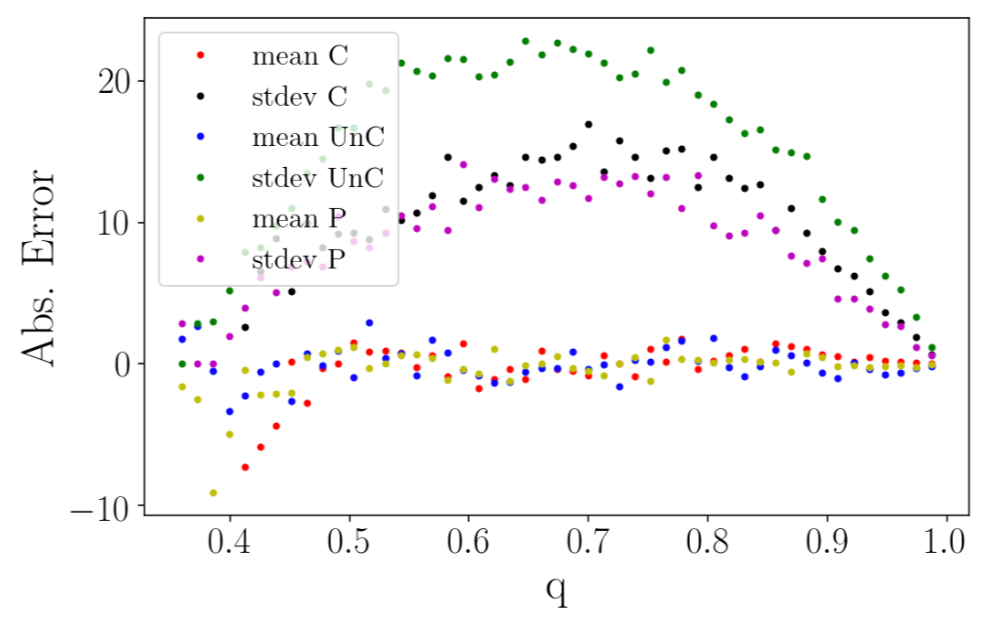
\includegraphics[width=\columnwidth]{variances.png}
\end{center}
\caption{
\zc{Ask Katerina for this data. Convert $\Lambda_s$ to $\tilde{\Lambda}$, then redo this image in xmgrace. Remove posterior eoss, Add a gridline at the maximum errors for both constrained and unconstrained, and maybe even show the relative errors as well? Probably remove the means as well.}
Absolute difference from the fit on $\tilde{\Lambda}$ from EoS variation in the binary Love universal relations plotted with varying mass ratio $q$.
Observe that the maximum systematic error attained for the constrained EoSs is $\sigma_{\tilde{\Lambda}}=10$ (this is found to be $20$ for the unconstrained EoSs).
This is negligible compared to the statistical errors accrued on paramter extraction from GW170817.\kc{Similar to an earlier comment, I think we should use the "posterior" EoSs since they were directly computed from the data.}
}
\label{fig:variances}
\end{figure}

%%%%%%%%%%%%%%%%%%%%%%%%% Begin Future Observations %%%%%%%%%%%%%%%%%%%%%%%%%%%%%%%%%%%%%%%%%%%%%%%%%%%%%%%%%%%%%%%%%%%%%%%%%%%%%%%%%%%%%%%%%%%%%%%%%%%%%%%%%%%%%%%%%%%%%%%%%%%%%%%%%%%%%%%%%%%%%%%%%%%%%
\section{Impact on future observations}\label{sec:observations}
In this section, we estimate the feasibility of ultilizing improved universal relations in future binary NS merger events.
This estimate is aqcuired through a simple Fisher analysis~\cite{Finn:Fisher,Cutler:Fisher} which approximates the accuracy with which one can extract best-fit parameters $\theta^a$, given a prior template waveform.
For the remainder of the paper, we consider a template parameter vector consisting of:
\begin{equation}
\theta^a=(\ln{A},\phi_c,t_c,\ln{\mathcal{M}},\ln{\mathcal{\eta}},\chi_s,\chi_a,\tilde{\Lambda},\delta \tilde{\Lambda}),
\end{equation}
where $A \equiv \sqrt{\frac{2 \eta}{3 \pi^{1/3}}}$ is a normalized amplitude factor, $\eta \equiv m_1 m_2/M^2$ is the symmetric mass ratio with $m_{1,2}$ and $M$ being the individual and total masses, $\mathcal{M}=M \eta^{3/5}$ is the chirp mass, and $\chi_{s,a}=\frac{1}{2}(\chi_1+\pm\chi_2)$ are the symmetric and antisymmetric total spins, where $\chi_{1,2}$ are the NSs individual spins. 
Following Refs.~\cite{Cutler:Fisher,Berti:Fisher,Poisson:Fisher}, this method relies on the crude assumption of Gaussian prior distributions\footnote{Typically, the more valid assumption is a uniform prior distribution; an improvement made in a more detailed Bayesian analysis.}.
The resulting posterior distribution is Gaussian with root-mean-sqaure given by:
\begin{equation}
\Delta \theta^a=\sqrt{\Big( \tilde{\Gamma}^{-1}\Big)^{aa}}.
\end{equation}
Here, the Fisher matrix $\tilde{\Gamma}$ is defined by:
\begin{equation}
\tilde{\Gamma}_{ab} \equiv \Big( \frac{\partial h}{\partial \theta^a} \Big| \frac{\partial h}{\partial \theta^a}\Big) + \frac{1}{\sigma_{\theta^a}^2} \delta_{ab}
\end{equation}
where $h$ is the waveform template, $\sigma_{\theta^a}$ is the parameters' prior root-mean-square estimate, and the inner product is defined by:
\begin{equation}
(a|b) \equiv 2 \int^{\infty}_0\frac{\tilde{a}^*\tilde{b}+\tilde{b}^*\tilde{a}}{S_n(f)}df.
\end{equation}
In this analysis, we consider the ``PhenomD" waveform template~\cite{PhenomDI,PhenomDII} modified by tidal corrections shown in Ref.~\cite{Wade:tidalCorrections}.
Lastly, $S_n(f)$ is the spectral noise density for the given interferometer.

We begin by authenticating this approach by applying a Fisher analysis to GW170817, as observed by LIGO with O2 detector sensitivity\zc{cite}.
Further, we scale the luminosity distance such that the signal-to-noise-ratio ($SNR \equiv \rho$) is fixed to be $\rho=32.4$, as was found in GW170817.
We also assume low spin priors $|\chi| \leq 0.05$, as well as $\tilde{\Lambda} \leq 3000$ and $|\delta \tilde{\Lambda}| \leq 500$~\cite{Wade:LambdaPriors}.
The resulting posterior distribution on $\tilde{\Lambda}$ has a range of $\pm 276.99$ encompassing the $90\%$ credible levels.
We compare these results with the Bayesian analysis performed in Ref.~\cite{TheLIGOScientific:2017qsa,Abbott2018}, finding close agreement with the resulting $90\%$ credible region of $70 \leq \tilde{\Lambda} \leq 720$.
This confirms the approximate validity of this method, allowing a continuation of this analysis for future detectors.
\begin{figure}
\begin{center} 
\includegraphics[width=\columnwidth]{sensitivities.eps}
\end{center}
\caption{
Square root of of the spectral noise densities $\sqrt{S_n^A(f)}$ plotted for detectors ($A$): LIGO O2 (orange), aLIGO (green), a\texttt{++} (purple), Voyager (magenta), CE (red), and ET-D (blue) as interpolated from publicly available data\zc{cite}.
Spectral noise densities are plotted from $f_{\text{min}}=(23,10,10,7,1,1) \text{ Hz}$, respectively, to $f_{\text{max}}=1649 \text{ Hz}$.
Also shown is $2 \sqrt{f}$ multiplied by the amplitude of the PhenomD~\cite{PhenomDI,PhenomDII} waveform template, modified by tidal corrections from Ref.~\cite{Wade:tidalCorrections} used in our Fisher Analysis.
}
\label{fig:sensitivities}
\end{figure}

Next, we consider events identical to GW170817 detected on future design sensitivity upgrades and detectors $A \equiv ($O2, aLIGO, a\texttt{++}, Voyager, CE, ET-D$)$\zc{cite}, shown in Fig.~\ref{fig:sensitivities}, to determine if and when the statistical errors associated with parameter extraction of $\tilde{\Lambda}$ drop below the systematic EoS variation errors from using binary Love universal relations.
The process we use for each detector sensitivity $S_n^A(f)$ is as follows:
\begin{itemize}
\item Perform a Fisher analysis as outlined above using $S_n^A(f)$, while restricting the luminosity distance $D_L$ such that $\rho^{\text{O2}}_{\text{GW170817}}=32.4$ would be achieved on O2 sensitivity $S_n^{\text{O2}}(f)$.
This results in SNR $\rho^A_{\text{GW170817}}$ and statistical error $\sigma_\text{GW170817}^A$ accrued in the extraction of $\tilde{\Lambda}$ on detector $A$.
\item Generate a population of $N_A$ events corresponding to the expected binary NS merger detection rate for detector $A$, following the distribution $f=3 \rho_{\text{th}}^3/\rho^4$~\cite{Shutz:SNR,Chen:SNR} with a network SNR threshold of $\rho_{\text{th}}=8$.
This is calculated for the upper, central, and lower limits of the local binary NS coalescence rate density $R=1540^{+3200}_{-1220} \text{ Gpc}^{-3}\text{yr}^{-1}$~\cite{Abbott2017}, giving the rates shown in the second column of Table~\ref{tab:variances}.
\item Compute the population standard deviation given by:
\begin{equation}
\frac{1}{(\sigma_N^A)^2}=\sum_i^{N_A}\frac{1}{(\sigma_i^A)^2},
\end{equation}
where $\sigma_i^A$ is computed by the relations $\sigma_i^A \times \rho_i^A = \sigma_{\text{GW170817}}^A \times \rho_{\text{GW170817}}^A$.
\end{itemize}
The results are compiled in Table~\ref{tab:variances}, and shown graphically in Fig.~\ref{fig:stackedFisher} where $\sigma^A_{\text{GW170817}}$ and $\sigma^A_N$ are plotted as a function of $\rho^A_{\text{GW170817}}$ (the SNR as if GW170817 were detected on future detector $A$) for 5 future detector sensitivities.

\begin{table*}[ht!]
\centering
\caption{
Tabulated results for the estimated statistical errors on $\tilde{\Lambda}$ for the combined results of $N_A$ detections corresponding to the estimated upper, central, and lower limits of the binary NS merger detection rate $R$.
This is repeated for 5 future detector sensitivities: aLIGO, a\texttt{++}, Voyager, CE, and ET.
Below, $\rho^A_{\text{GW170817}}$ and $\sigma^A_{\text{GW170817}}$ correspond to the approximate SNR and $\sigma_{\tilde{\Lambda}}$ of GW170817 had it been observed by the future interferometer, and $\sigma^A_N$ corresponds to the final uncertainty on $\tilde{\Lambda}$ after $N_A$ detections on interferometer $A$.
It can be seen here that the statistical errors on $\tilde{\Lambda}$ become comparable with the systematics $\sigma_{\tilde{\Lambda}}=10$ from using improved binary Love relations from Voyager and on, indicating when it may be safe to utilize new universal relations.
Note the approximation for $\sigma^A_N$ under the O2 detector sensitivity is a poor estimate due to the small number of stacked events, $N_{\text{O2}}=1$, resulting in a high degree of randomness in population generation.
These results are shown graphically in Fig.~\ref{fig:stackedFisher}.
}\label{tab:variances}
%\begin{tabular}{ c || c c c c c c c c} 
%\hline
%Detector ($A$) & $N_A (\text{Lower})$ & $N_A (\text{Central})$ & $N_A (\text{Upper})$ & $\rho^A_{\text{GW170817}}$ & $\sigma^A_{\text{GW170817}}$ & $\sigma^A_N (\text{Lower})$ & $\sigma^A_N (\text{Central})$ & $\sigma^A_N (\text{Upper})$\\
%\hline
%\hline
%O2 & $1$ & $1$ & $1$ & $32.40$ & $168.40$ & $558.18$ & $393.24$ & $279.44$\\
%aLIGO & $23$ & $112$ & $344$ & $90.74$ & $75.44$ & $117.022$ & $42.89$ & $24.27$\\
%a\texttt{++} & $208$ & $1004$ & $3091$              & $180.95$ & $31.55$ &               $27.62$ & $13.36$ & $7.36$\\
%Voyager & $3854$ & $1.85 \times 10^4$ & $5.71 \times 10^4$ &              $428.89$ & $16.69$              & $8.57$ & $3.78$ & $2.16$\\
%ET-D & $3.98\times 10^5$ & $1.91\times 10^6$ & $5.89\times 10^6$ &                  $2807.45$ & $6.26$ &               $0.78$ & $0.35$ & $0.20$\\
%CE & $1.35\times 10^7$ & $6.50\times 10^7$ & $2.00\times 10^8$ &                 $1398.03$ & $4.85$ &                 $0.34$ & $0.16$ & $0.10$\\
%\hline
%\end{tabular}
\begin{tabular}{|c|@{\extracolsep{4pt}}c@{\extracolsep{0pt}}|c|@{\extracolsep{4pt}}C{1.7cm}@{\extracolsep{-2pt}}|C{1.7cm}|@{\extracolsep{-2pt}}C{1.7cm}@{\extracolsep{2pt}}|c|@{\extracolsep{0pt}}c@{\extracolsep{0pt}}|c|}
\cline{1-1}\cline{2-3}\cline{4-9}
    \multicolumn{1}{|c|}{\bfseries Detectors (A)} & \multicolumn{2}{|c|}{\bfseries GW170817} & \multicolumn{6}{|c|}{\bfseries Multiple events} \\
\cline{1-1}\cline{2-3}\cline{4-9}
\noalign{\smallskip}
\cline{2-3}\cline{4-6}\cline{7-9}
\multicolumn{1}{c}{} & \multicolumn{1}{|c|}{} & \multicolumn{1}{c|}{} & \multicolumn{3}{|c|}{} & \multicolumn{3}{|c|}{}
\\[-1em]
\multicolumn{1}{c}{}  &  \multicolumn{1}{|c|}{\multirow{2}{*}{$\rho^A_{\text{GW170817}}$}}  &  \multirow{ 2}{*}{$\sigma^A_{\text{GW170817}}$}  &  \multicolumn{3}{|c|}{$N_A$}  &  \multicolumn{3}{|c|}{$\sigma^A_N$}  \\
\cline{4-6}\cline{7-9}
\multicolumn{1}{c}{}  &  \multicolumn{1}{|c|}{}  &  \multicolumn{1}{c|}{}  &  \multicolumn{1}{|c|}{Low}  &  \multicolumn{1}{c|}{Central} &  \multicolumn{1}{c|}{High}  & \multicolumn{1}{|c|}{Low}  &  \multicolumn{1}{c|}{Central} &  \multicolumn{1}{c|}{High}\\
\cline{2-3}\cline{4-6}\cline{7-9}
\noalign{\smallskip}
\noalign{\smallskip}
\cline{1-1}\cline{2-3}\cline{4-6}\cline{7-9}
 O2  & \multicolumn{1}{|c|}{$32.40$}  & $168.40$ &  \multicolumn{1}{|c|}{$1$} & $1$ & $1$ & \multicolumn{1}{|c|}{$558.18$} & $393.24$ & $279.44$\\
\cline{1-1}\cline{2-3}\cline{4-6}\cline{7-9}
 aLIGO  & \multicolumn{1}{|c|}{$90.74$}  & $75.44$ &  \multicolumn{1}{|c|}{$23$} & $112$ & $344$ & \multicolumn{1}{|c|}{$117.022$} & $42.89$ & $24.27$\\
\cline{1-1}\cline{2-3}\cline{4-6}\cline{7-9}
 a\texttt{++}  & \multicolumn{1}{|c|}{$180.95$}  & $31.55$ &  \multicolumn{1}{|c|}{$208$} & $1004$ & $3091$ & \multicolumn{1}{|c|}{$27.62$} & $13.36$ & $7.36$\\
\cline{1-1}\cline{2-3}\cline{4-6}\cline{7-9}

\multicolumn{1}{|c|}{} & \multicolumn{1}{|c|}{} & \multicolumn{1}{c|}{} & \multicolumn{1}{|c|}{} & \multicolumn{1}{c|}{} & \multicolumn{1}{c|}{} & \multicolumn{1}{|c|}{} & \multicolumn{1}{c|}{} & \multicolumn{1}{c|}{}
\\[-1em]

 Voyager  & \multicolumn{1}{|c|}{$428.89$}  & $16.69$ &  \multicolumn{1}{|c|}{$3854$} & $1.85 \times 10^4$ & $5.71 \times 10^4$ & \multicolumn{1}{|c|}{$8.57$} & $3.78$ & $2.16$\\
\cline{1-1}\cline{2-3}\cline{4-6}\cline{7-9}

\multicolumn{1}{|c|}{} & \multicolumn{1}{|c|}{} & \multicolumn{1}{c|}{} & \multicolumn{1}{|c|}{} & \multicolumn{1}{c|}{} & \multicolumn{1}{c|}{} & \multicolumn{1}{|c|}{} & \multicolumn{1}{c|}{} & \multicolumn{1}{c|}{}
\\[-1em]

 ET-D  & \multicolumn{1}{|c|}{$2807.45$}  & $6.26$ &  \multicolumn{1}{|c|}{$3.98 \times 10^5$} & $1.91 \times 10^6$ & $5.89 \times 10^6$ & \multicolumn{1}{|c|}{$0.78$} & $0.35$ & $0.20$\\
\cline{1-1}\cline{2-3}\cline{4-6}\cline{7-9}

\multicolumn{1}{|c|}{} & \multicolumn{1}{|c|}{} & \multicolumn{1}{c|}{} & \multicolumn{1}{|c|}{} & \multicolumn{1}{c|}{} & \multicolumn{1}{c|}{} & \multicolumn{1}{|c|}{} & \multicolumn{1}{c|}{} & \multicolumn{1}{c|}{}
\\[-1em]

 CE  & \multicolumn{1}{|c|}{$1398.03$}  & $4.85$ &  \multicolumn{1}{|c|}{$1.35 \times 10^7$} & $6.50 \times 10^7$ & $2.00 \times 10^8$ & \multicolumn{1}{|c|}{$0.34$} & $0.16$ & $0.10$\\
\cline{1-1}\cline{2-3}\cline{4-6}\cline{7-9}
\end{tabular}
\end{table*}

Concluding, we find that the Voyager, ET, and CE detectors all exhibit enough uncertainty reduction that the systematics from using improved universal relations no longer become negligible in the error budget.
This implies that the use and further improvement of universal relations is justified for future binary NS merger detections.

%%%%%%%%%%%%%%%%%%%%%%%%% Begin Discussion %%%%%%%%%%%%%%%%%%%%%%%%%%%%%%%%%%%%%%%%%%%%%%%%%%%%%%%%%%%%%%%%%%%%%%%%%%%%%%%%%%%%%%%%%%%%%%%%%%%%%%%%%%%%%%%%%%%%%%%%%%%%%%%%%%%%%%%%%%%%%%%%%%%%%
\section{Conclusion and Discussion}\label{sec:conclusion}
The recent GW observation of binary NS merger GW170817 placed constraints on the supranuclear matter EoS for NSs.
We take advantage of this by generating a restricted set of spectral EoSs which agree with this observation to reduce uncertainties upon the extraction of tidal parameters from future GW events.
Important previous work by Yagi and Yunes~\cite{Yagi:ILQ,Yagi:binLove} found EoS-insensitive universal relations between symmetric and antisymmetric combinations of NS tidal deformabilities, which aid in the extraction of said tidal parameters.
We find an improvement upon these universal relations by a factor of 25\% for stars with mass below 1.7 solar masses\zc{check this number} by restricting to the EoSs constrained by GW170817.
In addition, we find that binaries consisting of one massive hyrid quark-hadron star, and one small-mass hadron star do not obey these universal relations -- explained by the large difference in $\tilde{\Lambda}$ displayed between the constituent stars.
Further, we analyze the impact of this improvement for future binary NS merger detections, as the current detector sensitivity is not yet small enough to accurately constrain $\tilde{\Lambda}$ enough for universal relations to make a difference.
We find that future interferometers Voyager, CE, and ET-D all experience statistical uncertainties upon the extraction of $\tilde{\Lambda}$ small enough to become comparable to the systemtic errors injected by using the improved universal relations, as depicted in Fig.~\ref{fig:stackedFisher} and Table~\ref{tab:variances}.
This indicates that the use and further improvement of universal relations is justified for future GW observations of binary NS merger events.

Future work on this subject includes the possible constraint on the EoS through the observation of super-massive NSs combined with the results of GW170817.
For example, recent millisecond pulsar discovery J1748-2021B~\cite{Freire:superMassiveNS} has mass $2.74 \pm 0.21$, with large error bars due to astronomical mismodeling.
If verified, this provides a possible avenue of EoS constraint via considering only spectrally generated EoSs which support maximum NS mass in agreeance with J1748-2021B.
\zc{Should we talk about this here?}
In addition, separate binary Love universal relations for hybrid star binaries should be investigated.

%%%%%%%%%%%%%%%%%%%%%%%%% Begin Acknowledgements %%%%%%%%%%%%%%%%%%%%%%%%%%%%%%%%%%%%%%%%%%%%%%%%%%%%%%%%%%%%%%%%%%%%%%%%%%%%%%%%%%%%%%%%%%%%%%%%%%%%%%%%%%%%%%%%%%%%%%%%%%%%%%%%%%%%%%%%%%%%%%%%%%%%%
\section*{Acknowledgments}\label{acknowledgments}
K.Y. would like to acknowledge networking support by the COST Action
GWverse CA16104. \zc{everyone elses acknowledgments. Which grant am I funded by?}

%%%%%%%%%%%%%%%%%%%%%%%%% Begin Bibliography  %%%%%%%%%%%%%%%%%%%%%%%%%%%%%%%%%%%%%%%%%%%%%%%%%%%%%%%%%%%%%%%%%%%%%%%%%%%%%%%%%%%%%%%%%%%%%%%%%%%%%%%%%%%%%%%%%%%%%%%%%%%%%%%%%%%%%%%%%%%%%%%%%%%%%
%\clearpage
\bibliography{Zack}
\end{document}

